% !TeX spellcheck = cs_CZ
%---------------------------------------------------------------------------------------------------
% mai2ch04.tex
%---------------------------------------------------------------------------------------------------
\setchaptertoc
\chapter{Obyčejné diferenciální rovnice}\label{mai:IIchapIV}

  V partii \ref{part:MAI} jsme se seznámili s funkcemi, o jejich užitečnosti nepochybujeme, neboť
  jsme se již přesvědčili, že se s nimi setkáváme takřka na každém kroku. Vyjadřují totiž
  jednoduchým způsobem vzájemnou souvislost veličin, a nejen fyzikálních. Známe-li například funkci
  vyjadřující závislost polohy tělesa na čase, můžeme zjistit, kde těleso v daném okamžiku bylo, je,
  nebo bude. Známe-li funkce, které popisuji časový vývoj cen a platů, můžeme snadno zjistit, zda za
  stejný peníz, za který dnes dostaneme deset housek, koupíme za rok dvacet, nebo jen dvě. Příroda,
  a ani ekonomika či politika, však nejsou natolik průhledné, aby nám takové závislosti předestřely
  přímo. Poskytují pouze informace o jejich změnách, a to ještě ukryté ve speciálních rovnicích,
  zvaných \emph{diferenciální}. Jde-li o neznámou reálnou funkci nebo soubor funkcí závislých na
  jedné reálné proměnné, třeba na čase, hovoříme o obyčejných diferenciálních rovnicích. Přesněji
  řečeno, diferenciální rovnice vyjadřuje matematickou formou zákon platný pro hledanou funkci a
  její derivace prvního nebo i vyšších řádů. Takovou funkcí času může být například i množství látky
  při chemických reakcích, mohutnost populace živočichů, kurz eura, cena akcií na burze, rychlost
  pohybu těles, teplota atd. Ve fyzice a chemii jsou diferenciální rovnice dány fyzikálními či
  chemickými zákony, v ekonomii nebo biologii se objevují v různých modelech, odpovídajících více či
  méně skutečnosti. Uveďme si několik příkladů, na nichž si vysvětlíme základní terminologii, která
  je s problematikou diferenciálních rovnic spojena.
  
  Doplňková literatura pro studium této partie je například: \cite[s.~217]{Musilova2012MA2} a 
  \cite[s.~426]{Brabec1989}. Pro procvičení elementárních metod řešení konkrétních rovnic je vhodná 
  sbírka řešených příkladů \cite[s.~348]{Jirasek1989}.
  
  %--Příklad s hlemýžděm------------------------------------------
      % !TeX spellcheck = cs_CZ
% Musilova2009MA2
\begin{mdframed}[style=mdexam]
  \begin{example}\label{mai:exam084}
    \textbf{Pohyb po přímce}\newline
    Hlemýžď se pohybuje po přímce od kopretiny k pampelišce stálou rychlostí \(v_0 =
    \qty{2}{\mm\per\s}\). V počátečním okamžiku \(t = 0\) byl ve vzdálenosti \(s_0 = \qty{10}{\mm}\)
    od kopretiny. Jaká bude jeho vzdálenost od kopretiny v libovolném okamžiku \(t\geq0\)? Na tuto
    otázku by jistě snadno odpověděl i žák první třídy. Ukažme si však, že úlohu lze také vyjádřit
    pomocí diferenciální rovnice. Vzdálenost \(s(t)\) je hledanou funkcí jedné proměnné, a to času
    \(t\). Rychlost \(v_0\) rovnoměrného přímočarého pohybu je časovou derivací vzdálenosti.
    Získáváme tedy rovnici

    {\centering
     \captionsetup{type=figure}
     \luafigure[0.7]{mai_fig055.png}
     \captionof{figure}{Hlemýžď pohybující se po přímce od kopretiny k pampelišce 
                       \cite[s.~217]{Musilova2012MA2}}
     \label{mai:fig055}
    \par}
    
    \begin{equation}\label{mai:eq076}
      \der{s(t)}{t} = v_0.
    \end{equation}

    Již jsme se zmínili, že rovnice obsahující neznámou reálnou funkci jedné reálné proměnné a její
    derivace obecně i vyššího řádu se nazývá obyčejnou diferenciální rovnicí. Každá z funkcí, které
    rovnici splňují, se nazývá jejím řešením. Řád rovnice je určen nejvyšší derivací, která se v
    rovnici vyskytuje, v našem příkladu jde tedy o rovnici prvního řádu.

    {\centering
     \captionsetup{type=figure}
     \luafigure[1]{mai_fig054.png}
     \captionof{figure}{Graf řešení počáteční úlohy (\ref{mai:eq077}).}
     \label{mai:fig054}
    \par}
    
    Řešení rovnice (\ref{mai:eq076}) snadno \uv{uhodneme}. Bude jím každá funkce
    \begin{equation*}
      s(t) = v_0t +C,
    \end{equation*}
    kde \(C\) je libovolné reálné číslo. Funkce, které jsou řešením rovnice, mají stejný charakter a
    jsou odlišeny pouze číselnou hodnotou \(C\), tvoří soubor, který se nazývá \textbf{obecné řešení
    rovnice}. Ze všech funkcí, které vyhovují rovnici (\ref{mai:eq076}), však skutečný pohyb
    hlemýždě popisuje právě jedna. Abychom ji našli, potřebujeme určit správnou hodnotu \(C\). K
    jejímu zjištění stačí, abychom věděli, jaká byla poloha hlemýždě v jediném okamžiku. Jestliže
    jsme například začali měřit čas ve chvíli, kdy byl hlemýžď ve vzdálenosti \(s_0\) od kopretiny,
    máme tzv. \textbf{počáteční podmínku} \(s(0) = s_0\). Pomocí ní můžeme z nekonečně mnoha funkcí
    obecného řešení vybrat jediné \textbf{partikulární řešení}. V našem případě to bude funkce
    \(s(t) = v_0t + s_0\). Naše rovnice společně s počáteční podmínkou, tj.
    \begin{equation}\label{mai:eq077}
      \der{s(t)}{t} = v_0, \qquad s(0) = s_0,
    \end{equation}
    představuje tzv. \textbf{počáteční úlohu}. Její řešení je v grafu na obrázku \ref{mai:fig054}
    vyznačeno červeně, modře jsou vyznačena některá další partikulární řešení. Dokážete určit, jaké
    počáteční úloze odpovídají?
  \end{example}
\end{mdframed}
  %---------------------------------------------------------------
  Ve většině příkladů, se kterými se setkáme, bude mít počáteční úloha právě jedno řešení, jak tomu
  je v případě hlemýždě. Jestliže je nějaká funkce, definovaná na intervalu \((a,b)\), řešením
  počáteční úlohy, pak každá funkce, kterou vytvoříme zúžením původního řešení na „menší“ interval,
  bude opět rovnici splňovat. My však máme \emph{„právě jedním řešením“} na mysli tzv. \textbf{úplné
  řešení}, tj. takové, které není zúžením žádného jiného, a tak řešení lišící se pouze definičním
  oborem nebudeme považovat za odlišná. Jak uvidíme později, vyskytnou se však také příklady, kdy
  počáteční úloha nemá žádné řešení, nebo jich má naopak nekonečně mnoho.

  %--Příklad s koupelnou------------------------------------------
      % !TeX spellcheck = cs_CZ
% Musilova2009MA2
\begin{mdframed}[style=mdexam]
  \begin{example}\label{mai:exam085}
    \textbf{Příklad s koupelnou}\newline
      V koupelně o celkovém objemu \(V = \num{12000}\) litrů byl nainstalován větrák, jehož výkon je
      \(P = \num{400}\) litrů za minutu. Položme si otázku: Jaká je optimální doba, na kterou je
      třeba nastavit časový spínač, aby větrák neběžel příliš dlouho a přitom se vyměnil všechen
      vzduch v místnosti? A je to vůbec možné? Může se opravdu vzduch vyměnit všechen? Přemýšlejme o
      této situaci důkladněji. Označme \(c(t)\) funkci popisující okamžitou objemovou koncentraci
      „původního vzduchu“ v místnosti, tj. poměr objemu původního vzduchu ku objemu místnosti. (V
      okamžiku zapnutí větráku, tj. pro \(t = 0\), je \(c(0) = c_0 = 1\), v okamžiku, kdy bude
      původní vzduch zcela vyčerpán, pokud to vůbec nastane, bude \(c = 0\).) V intervalu \([t,t +
      \Delta t]\) větrák odčerpá \(P\Delta t\) litrů vzduchu celkem, z toho množství starého vzduchu
      činí \(c(t)P\Delta t\) a jeho podíl na celkovém množství vzduchu je \(c(t)P\Delta t/V\). Tato
      hodnota představuje pro velmi malé \(\Delta t\) \textbf{úbytek} koncentrace starého vzduchu v
      koupelně v časovém intervalu \([t, t + \Delta t]\), tj.
      \begin{equation*}
        \Delta c(t) = - \frac{c(t)P\Delta t}{V} \Rightarrow 
        \dfrac{\Delta c(t)}{\Delta t} = - \dfrac{P}{V}c(t)
      \end{equation*}
      
      (uměli bychom vysvětlit záporné znaménko?). Získáváme rovnici
      \begin{equation}\label{mai:eq078}
        \der{c(t)}{t} = - \dfrac{P}{V}c(t)
      \end{equation}
      Dosazením snadno ověříme, že řešením rovnice (\ref{mai:eq078}) je každá funkce
      \begin{equation*}
        c(t) = Ke^{-\frac{Pt}{V}},
      \end{equation*}

      {\centering
      \captionsetup{type=figure}
      \luafigure[1]{mai_fig056.png}
      \captionof{figure}{Graf řešení úlohy s koupelnou.}
      \label{mai:fig056}
      \par}
      
      kde \(K\) je libovolné číslo. Jeho konkrétní hodnotu pro náš případ určíme z počáteční
      podmínky \(c(0) = 1\), tj. \(K = 1\). A vida, pokud jsme počítali správně, můžeme usoudit, že
      koncentrace původního vzduchu neklesne na nulovou hodnotu nikdy. Naše řešení samozřejmě
      nevylučuje použití časového spínače - rozumně bychom mohli například požadovat, aby
      koncentrace původního vzduchu klesla na hodnotu \(c(\tau) = \num{0.1}\). Hledaná doba bude \(t
      =\frac{P}{V}\ln(1/c(\tau)) =\qty{69}{\minute}\). Řešení naší počáteční úlohy je v grafu na
      obrázku \ref{mai:fig056} vyznačeno červeně. Jakým počátečním úlohám odpovídají modré křivky?
  \end{example}
\end{mdframed}
  %---------------------------------------------------------------
  
  \begin{note}
    „Větrací“ rovnice, diskutovaná v předchozím případě, se ve fyzice objevuje poměrně často. Někdy
    je nazývána lineárním diferenciálním zákonem. Narazíme na ni vždy, když je rychlost změny nějaké
    veličiny (její první derivace) přímo úměrná veličině samotné. Tak například při rozpadu
    radioaktivních jader dospějeme k rovnici \(\der{N(t)}{t} = -\lambda N(t)\), kde \(N(t)\) je
    počet radioaktivních jader ve vzorku v okamžiku \(t\) a \(\lambda\) je \textbf{rozpadová
    konstanta}. Při zkoumání absorpce rentgenového záření v látce získáme rovnici \(\der{I(x)}{x} =
    -\mu I(x)\), kde \(I(x)\) je intenzita v hloubce \(x\) pod povrchem a \(\mu\) je lineární
    \textbf{koeficient absorpce}. S oběma příklady jsme se již setkali v partii \ref{part:MAI}.
    Zkusme si vzpomenout na další příklady lineárních diferenciálních zákonů.
  \end{note}

  %--Příklad o sáňkování------------------------------------------
      % !TeX spellcheck = cs_CZ
% Musilova2009MA2
\begin{mdframed}[style=mdexam]
  \begin{example}\label{mai:exam086}
    \textbf{Příklad o sáňkování}\newline
    Kdo bude rychlejší na sáňkách? Tatínek o hmotnosti \(M\), nebo Pepíček s Mařenkou o hmotnosti
    \(m\)? Každý fyzik hned namítne, že tíhové zrychlení, které určuje rozjezd sáněk, na hmotnosti
    nezávisí. Z praxe však víme, že tatínkové bývají rychlejší. Jak to? Zřejmě proto, že sáňkování
    ve vakuu není obvyklé. Kromě průmětu tíhové síly do nakloněné roviny (\(F_1 = Mg\sin\alpha\)),
    který „nás urychluje", jsme brzděni silou odporu prostředí. V jednoduchém přiblížení ji můžeme
    předpokládat ve tvaru \(F_2 = -Cv^2\). Konstanta \(C\) závisí na tvaru a rozměrech pohybujícího
    se objektu a na hustotě vzduchu. Pro jednoduchost předpokládáme, že je stejná u tatínka i
    Pepíčka. Fyzikální zákon \(Ma= F_1 + F_2 = Mg\sin\alpha - Cv^2\)

    {\centering
    \captionsetup{type=figure}
    \luafigure[1]{mai_fig057.jpg}
    \captionof{figure}{Ladův obrázek dětí na sáňkách.}
    \label{mai:fig057}
    \par}

    například pro tatínka můžeme přepsat na diferenciální rovnici takto:
    \begin{equation}\label{mai:eq079}
      M\der{v}{t} = Mg\sin\alpha - Cv^2
    \end{equation}
    
    Hledanou funkcí je nyní časová závislost rychlosti, jako počáteční podmínku budeme uvažovat, že
    rychlost v čase \(t = 0\) byla nulová. Řešením této počáteční úlohy je funkce
    \begin{align*}
      v(t) &= \sqrt{\dfrac{Mg\sin\alpha}{C}}
              \left[\dfrac{e^{2t\sqrt{\dfrac{Cg\sin\alpha}{M}}}-1}
                          {e^{2t\sqrt{\dfrac{Cg\sin\alpha}{M}}}+1}
              \right]                                                                           \\
          &= \sqrt{\dfrac{Mg\sin\alpha}{C}}\tanh\left(t\sqrt{\dfrac{Cg\sin\alpha}{M}}\right).
    \end{align*}
    Graf takovéto závislosti pro dvě různé hmotnosti \(M = \qty{100}{\kg}\) (červená) a \(m =\qty{10}
    {\kg}\) (modrá) vidíme na obrázku \ref{mai:fig057}. (Poměr hmotností byl takto zvolen pro
    zvýraznění rozdílnosti výsledků - každému je zřejmé, že mimino samo sáňkovat nemůže.) Další
    hodnoty: \(\alpha = \ang{20}\), \(g = \qty{10}{\m\per\square\s}\), \(C =
    \qty{1.00}{N\m^2s^{-2}}\). Na obrázku \ref{mai:fig058} si všimněme, že rychlost se nejprve

    {\centering
    \captionsetup{type=figure}
    \luafigure[1]{mai_fig058.png}
    \captionof{figure}{Graf řešení úlohy o sáňkování. \cite[s.~221]{Musilova2012MA2}}
    \label{mai:fig058}
    \par}

    poměrně prudce zvyšuje, ale poté se asymptoticky blíží k tzv. \textbf{mezní rychlosti} \(v_{max}
    = Mg\sin\alpha\). Mezní rychlost odpovídá situaci, kdy se síly \(F_1\) a \(F_2\) „vyrovnají“.
    (Taková situace však nenastane, je pouze limitním případem pro \(t \rightarrow \infty\).) 
  \end{example}
\end{mdframed}
  %---------------------------------------------------------------
  \begin{note}
    Zamysleme se také nad tím, jak jsme z vyjádření funkce \(v(t)\) pomocí exponenciálních funkcí 
    získali elegantnější výraz s hyperbolickou tangentou. Pro připomenutí hyperbolických funkcí se 
    můžeme vrátit k odstavci 2.1.8 partie \ref{part:MAI}.
  \end{note}
  
  Na uvedených příkladech jsme se mohli přesvědčit, že porozumění některým realistickým dějům
  vyžaduje umět sestavit a řešit diferenciální rovnice. Problémy, se kterými se v životě setkáváme,
  však obvykle vedou k rovnicím mnohem komplikovanějším. Proto často používáme aproximací a skutečný
  svět si poněkud „idealizujeme". Tak například v úloze s koupelnou jsme předpokládali, že vzduch v
  místnosti je vždy dokonale promíchán, v úloze o sáňkování jsme pro odporovou sílu použili pouze
  přibližný zákon a zanedbali třecí sílu. Často se setkáme s rovnicemi, které dokážeme řešit pouze
  numerickými metodami za pomoci počítačů. Aproximativní přístupy tedy mohou vstupovat do popisu
  vývoje reálných systémů pomocí diferenciálních rovnic dvojím způsobem. Poprvé již při samotném
  sestavení diferenciálních rovnic, podruhé při jejich řešení.
  
  V této kapitole se budeme věnovat některým typickým situacím, kdy je možné získat řešení
  diferenciálních rovnic analytickými metodami, zjednodušeně řečeno „tužkou na papíře“. Proč se
  omezujeme na některé typické situace“? Protože problematika diferenciálních rovnic obsahuje ještě
  další úskalí. Řečeno s mírnou nadsázkou, existuje totiž nepřeberné množství různých typů
  diferenciálních rovnic, dokonce už v případě rovnic prvního řádu, které při řešení vyžadují takřka
  \uv{individuální přístup}. I když samozřejmě v teorii diferenciálních rovnic existuje řada
  obecných výsledků společných určité širší skupině diferenciálních rovnic, není možné formulovat
  nějaký \uv{univerzální} postup, který by vedl k řešení kterékoli z nich. V praxi je proto třeba
  naučit se rozpoznat jednotlivé typy obyčejných diferenciálních rovnic a zvolit pro jejich řešení
  vhodnou metodu. Ne nadarmo se proto textům o diferenciálních rovnicích říká „kuchařky“, aniž by to
  mělo hanlivý nádech. (Vznešenější slovo pro „kuchařku“ je „příručka“. Pokud jde o problematiku
  obyčejných diferenciálních rovnic, je takovou moderní příručkou kniha \cite{PolyaninZaitsev},
  která na více než osmi stech stran obsahuje přes 6 200 rovnic s řešeními!
  
  \twocolumn[\section{Diferenicální rovnice vyskytující se kolem nás}\label{mai:IIchapIVsecI}]
    V tomto odstavci jsou zařazeny motivační příklady ukazující, že diferenciální rovnice se
    skutečně objevují v různých vědních oborech. Rovnice jsou většinou uvedeny bez řešení, ale jsou
    doplněny alespoň odkazy ve kterých lze najít mnohem více informací, které jdou za rámec této
    partie o obyčených diferenciálních rovnicích. Stejně jako v předchozích příklad, řada
    fyzikálních principů má tvar výroku, resp. vztahu mezi jistými veličinami (funkcemi) a jejich
    změnami, vztaženými ke zvoleným nezávisle proměnným (pa\-ra\-me\-trům) (\emph{čas, souřadnice}).
    Je to přirozené, neboť (\emph{okamžité}, či \emph{okální}) změny se nejlépe vystihují pomocí
    derivací. Takový zákon má pak charakter vztahu mezi uvažovanými veličinami a jejich derivacemi. 
    
    \begin{mdframed}[style=mdnote] 
      V matematických textech o obyčejných diferenciálních rovnicích se označuje nezávisle proměnná 
      obvykle symbolem \(x\), neznámá funkce \(y = y(x)\) nebo \(y = f(x)\) a její derivace 
      čárkami, tj. \(y'(x)\), \(y''(x)\) nebo \(y' = f'(x)\), \(y" = f''(x)\) atd. V mnoha 
      fyzikálních i jiných praktických situacích však bývá nezávisle proměnnou čas \(t\) a hledáme 
      závislost veličiny \(x = x(t)\) na čase. Tohoto značení budeme velmi často používat, přičemž 
      první, resp. druhou derivaci funkce \(x(t)\) budeme podle zvyklosti zavedené ve fyzice 
      vyznačovat pomocí tečky, resp. dvou teček nad symbolem \(x\),
      \begin{equation*}
        \dot{x}(t) = \der{x}{t}, \qquad \ddot{x}(t) = \dder{x}{t}.
      \end{equation*}
      Pro větší přehlednost zápisu budeme často vynechávat argument \(t\) v závorce, \(\dot{x} = 
      \dot{x}(t)\). Nebudeli řečeno jinak, předpokládáme, že všechny funkce jsou spojité, případně 
      i diferencovatelné na celém svém definičním oboru nebo alespoň na jistém oboru, který je jeho 
      podmnožinou. Při práci s podílem funkcí budeme automaticky předpokládat, že jmenovatelem je 
      funkce, která je nenulová ve všech bodech uvažovaného intervalu.      
    \end{mdframed}
    
    \subsection{Diferenciální rovnice v mechanice}
      \textbf{Druhý Newtonův pohybový} zákon pro hmotný bod, který nabývá tvaru
      \begin{equation*}
        m\vec{a} = \vec{F}
      \end{equation*}
      skrývá soustavou \emph{tří diferenciálních rovnic druhého řádu}. Složky zrychlení \(\vec{a}(t)
      = (a_x(t), a_y(t), a_z(t)) = (\ddot{x}(t), \ddot{y}(t), \ddot{z}(t))\) jsou totiž druhými
      derivacemi složek polohového vektoru \(\vec{r}(t) = (x(t), y(t), z(t))\) podle času, vektor
      výslednice sil působících na hmotný bod je obecně funkcí jeho polohy a rychlosti, a často také
      explicitní funkcí času. Platí tedy \(\vec{F} = \vec{F}(\vec{r},\vec{v},t)\). Rozepíšeme-li
      druhý Newtonův zákon do složek, dostaneme
      \begin{align*}
        m\ddot{x} & = F_x(x,y,z,\dot{x}, \dot{y}, \dot{z}, t),        \\
        m\ddot{y} & = F_y(x,y,z,\dot{x}, \dot{y}, \dot{z}, t),        \\
        m\ddot{z} & = F_z(x,y,z,\dot{x}, \dot{y}, \dot{z}, t)
      \end{align*}
      Řešením této soustavy je časová závislost \(\vec{r} = (x(t), y(t), z(t))\) polohového vektoru
      hmotného bodu. Je \emph{parametrickým vyjádřenim křivky}, po které se hmotný bod v prostoru
      pohybuje, nazývá se \emph{trajektorií} pohybu.Zadáním počáteční polohy \(\vec{r}_0 = (x(t_0),
      y(t_0), z(t_0))\) a počáteční rychlosti \(v_0 = (\dot{x}(t_0), \dot{y}(t_0), \dot{z}(t_0))\)
      například v okamžiku \(t_0 = 0\) ziskáme \textbf{počáteční úlohu}. (Soustava obsahuje druhé
      derivace neznámých funkci \(x(t)\), \(y(t)\) a \(z(t)\), proto potřebujeme dvě podminky pro
      každou z nich.) 
      
      Zapišme takový příklad konkrétní soustavy: Na planetu o hmotnosti \(m\) působí Slunce o
      hmotnosti \(M\) silou \(\vec{F}_g\) danou Newtonovým gravitačním zákonem. Tentokrát však jde o
      tzv. „silový zákon", který popisuje gravitační interakci planety a Slunce. Umístíme-li počátek
      soustavy souřadnic do hmotného bodu představujícího Slunce, platí
      \begin{equation*}
        \vec{F}_g = - \dfrac{\kappa mM\vec{r}}{r^3} 
                  = - \dfrac{\kappa mM}{(x^2+y^2+z^2)^{\frac{3}{2}}}(x, y, z)
      \end{equation*}
      kde \(\kappa =  \SI{6.67e-11}{\N\m^2\kg^{-2}}\) je jednou z univerzálních fyzikálních
      konstant, nazývanou gravitační konstanta. Za předpokladu, že zanedbáme pohyb Slunce a
      gravitační působení planet a ostatních těles, má soustava rovnic vyjadřující druhý Newtonův
      zákon pro planetu tvar 
      \begin{subequations}
        \begin{empheq}[box=\widefbox]{align*}
          m\ddot{x} & = - \kappa mM \dfrac{x}{(x^2+y^2+z^2)^{\frac{3}{2}}},        \\
          m\ddot{y} & = - \kappa mM \dfrac{y}{(x^2+y^2+z^2)^{\frac{3}{2}}},        \\
          m\ddot{z} & = - \kappa mM \dfrac{z}{(x^2+y^2+z^2)^{\frac{3}{2}}}
        \end{empheq}
      \end{subequations}

      Nalézt řešení této soustavy znamená „vydolovat" z ní, při daných počátečních podmínkách,
      konkrétní tvar funkcí \(x(t)\), \(y(t)\) a \(z(t)\). Zrovna tato úloha není příliš jednoduchá.
      Postup při jejím řešení, který lze usnadnit použitím fyzikálních „triků”, si ukážeme později. 

    \subsection{Diferenciální rovnice v chemii}
      Uvažujme o chemické reakci, při které se ze dvou látek \(A\) a \(B\) syntetizuje látka \(C\).
      Na jeden gram výsledné látky je zapotřebí \(p\) gramů látky \(A\) a \(1 - p\) gramů látky
      \(B\). Smícháme \(a\) gramů látky \(A\) s \(b\) gramy látky \(B\). Na počátku je hmotnost
      látky \(C\) nulová, její hodnotu v čase \(t\) označíme \(x(t)\). Rychlost chemické reakce, tj.
      změna hmotnosti látky \(C\) s časem, je v rámci nejjednoduššího modelu rovna veličině \((a -
      px) (b - (1 - p)x)\). Vidíme, že při zvětšujícím se množství výsledné látky bude rychlost
      reakce klesat. Ve výsledku se projeví i to, jaké množství výchozích látek smícháme, resp. jak
      se jejich poměr \(\dfrac{a}{b}\) bude lišit od „ideálního" poměru \(\dfrac{p}{1-p}\). Rovnice
      popisující reakci je diferenciální rovnicí prvního řádu pro časovou závislost \(x(t)\)
      hmotnosti látky \(C\)
      \begin{equation*}
        \boxed{\dot{x} = (a - px)(b - (1-p)x)}\, ,
      \end{equation*}
      s počáteční podmínkou \(x(0) = 0\). K této rovnici se ještě hodí poznamenat, že je příkladem
      (i když velmi speciálním) známé \textbf{Riccatiovy rovnice}, která má uplatnění i v
      praktických disciplínách, například v elektrotechnice nebo v oblasti automatického řízení.
      Přestože má nevinně vypadající obecný tvar \(x(t) = h(t) + f(t)x +g(t)x^2\), \(h(t) \neq 0\),
      \(g(t) \neq 0\), je tak trochu „zrádná“. Její řešení se totiž nemusí podařit zapsat pomocí
      elementárních funkcí. 
    
    \subsection{Diferenciální rovnice v biologii}
      Uvažujme o vlkovi a zajíci. Předpokládáme-li, že zajíc má vždycky co žrát (trávy je všude
      dost), bude nárůst počtu zajíců úměrný jejich okamžitému počtu (čím více je zajíců, tím více
      dalších se narodí). Zároveň jsou zajíci požíráni vlky a jejich úbytek je úměrný jak počtu
      vlků, tak počtu jich samých (čím více je zajíců, tím více jich každý věčně hladový vlk chytí a
      sežere, čím více je vlků, tím více zajíců sežerou). Co se vlků týče, ty nikdo nesežere, ale
      budou umírat hladem, jestliže nebude dostatek zajíců. Nárůst počtu vlků je tedy úměrný jak
      počtu vlků, tak počtu zajíců, kdežto úbytek je úměrný pouze počtu vlků. Získáváme soustavu
      dvou diferenciálních rovnic

      \begin{subequations}
        \begin{empheq}[box=\widefbox]{align*}
          \dot{z} &= \alpha z - \beta zv,     \\
          \dot{v} &= \gamma v + \delta zv,
        \end{empheq}
      \end{subequations}

      kde funkce \(z(t)\) resp. \(v(t)\) vyjadřují časovou závislost počtu zajíců, resp. vlků.
      Konstanty \(\alpha\), \(\beta\), \(\gamma\), \(\delta\) lze určit dlouhodobým pozorováním. 
      \begin{note}
        Pokud někoho napadlo, že zajíci i vlci se také rodí i umírají „přirozenou cestou“, má
        pravdu. Tato skutečnost je v našem jednoduchém modelu zahrnuta. Přirozený přírůstek či
        úbytek zajíců i vlků je také úměrný jejich okamžitému počtu, a je tedy respektován
        empirickými hodnotami \(\alpha\), \(\gamma\).
      \end{note}
      
      Tato soustava nelineárních diferenciálních rovnic se nazývá \textbf{Lotkova-Volterrova}. 
      Existence triviálního, tj. identicky nulového řešení, odpovídajícího situaci, kdy žádný zajíc 
      ani vlk neexistují je zřejmá na první pohled. Rovnice má však také netriviální řešení, které 
      si později ukážeme. 
      
      Obdobným příkladem z biologie je situace, kdy diferenciální rovnice popisuje časový průběh
      vývoje jedné populace. Řekněme, že jde o populaci bakterií, jejíž velikost v závislosti na
      čase je dána funkcí \(P(t)\). Při vývoji hrají roli dva nezávislé faktory, jeden způsobuje
      růst populace a druhý souvisí s omezeními danými prostředím. Představme si situaci tak, že bez
      omezujících vlivů prostředí by populace narůstala podle lineárního diferenciálního zákona, tj.
      derivace \(\dot{P}(t)\) hledané funkce \(P(t)\) by byla v každém okamžiku přímo úměrná hodnotě
      \(P(t)\), konstantu úměrnosti \(R\) nazvěme \emph{faktorem růstu}. Okolní prostředí však
      znemožňuje neomezené narůstání funkčních hodnot \(P(t)\). Růst je totiž modifikován tak, že se
      anuluje v okamžiku, kdy je dosaženo \uv{povolené} hodnoty \(P_{max} = K\), tj. když hodnota
      funkce \(P(t)\) dosáhne úrovně \emph{nosné kapacity} \(K\). Odpovídající diferenciální rovnice
      je opět nelineární a zní
      \begin{equation*}
        \boxed{\dot{P} = RP\left(1 - \dfrac{P}{K}\right)}
      \end{equation*}
      Nazýváme ji \textbf{logistickou rovnicí} a rovněž se ji naučíme vyřešit.
      
    \subsection{Diferenciální rovnice v ekonomii}
      V novinách se občas objeví zpráva, že míra inflace klesá. Od obyvatelstva se očekává, že to
      bude interpretovat jako pozitivní jev v naší ekonomice. Je tomu tak skutečně? Označme jako
      \(h(t)\) funkci popisující vhodným způsobem „kupní sílu“ koruny v závislosti na čase (název
      funkce \(h(t)\) jsme dali do uvozovek, neboť skutečná situace je z pohledu ekonomiky
      složitější a nezávisí pouze na inflaci). Její záporně vzatou derivaci \(\mu = -\der{h(t)}{t} =
      -h\) nazýváme mírou inflace. Proč znaménko minus? Pokud je funkce \(h(t)\) klesající, tj.
      kupní síla peněz se snižuje, je její derivace záporná. O míře inflace se však při znehodnocení
      kupní síly hovoří jako o kladné veličině. Jestliže míra inflace podle novinářů klesá, je její
      derivace \(\mu(t)\) záporná. Předpokládejme pro jednoduchost, že velikost této derivace je
      stálá. Druhá derivace neznámé funkce \(h(t)\) je tedy kladná konstantní hodnota, označme ji
      třeba \(A\), \(A > 0\). Dostáváme velmi jednoduchou diferenciální rovnici
      \begin{equation*}
        \ddot{h} = A.
      \end{equation*}
      kterou můžeme okamžitě vyřešit. Vyhovují jí všechny funkce tvaru
      \begin{align*}
        h(t) &= \dfrac{1}{2}At^2 -\mu_1(t) + h_0 \\
             &= \dfrac{A}{2}\left(t-\dfrac{\mu_1}{A}\right)^2+\left(h_0-\dfrac{\mu_1^2}{2A}\right), 
      \end{align*}
      přičemž význam konstant \(h_0\) a \(\mu_1\) je takový, že \(h_0 = h(0) > 0\) představuje
      počáteční kupní sílu peněz, \(\mu_1 = -\dot{h}(0) = \mu(0) > 0\) je počáteční míra inflace.
      Grafem řešení rovnice je parabola, která má konvexní průběh, neboť \(\ddot{h} = A > 0\). Její
      vrchol (minimum) odpovídá bodu \(t_0 = \mu_1/A\). V tomto okamžiku dosáhne míra inflace nulové
      hodnoty. V časovém intervalu \([0, t_0]\) tedy kupní síla našeho platu i přes optimisticky
      vypadající novinovou zprávu stále klesá, tento pokles se však postupně zmírňuje a v okamžiku
      \(t_0\) je nulový - od tohoto okamžiku již neplatí původní tvrzení, že míra inflace klesá
      (nemůže být totiž záporná, nešlo by o inflaci). Interval \([0, t_0]\) je tedy oborem, na
      kterém je řešení diferenciální rovnice pro daný případ relevantní, i když řešení rovnice
      existuje na celé reálné ose.
      
      Jiný ekonomický model může představovat ,spojité" úročení vkladu v bance. Předpokládejme, že
      úrok činí konstantní část \(k\), obvykle několik procent, okamžité výše vkladu. Je-li výše
      vkladu popsána funkcí \(x(t)\), pak
      \begin{equation*}
        \dot{x} = kx.
      \end{equation*}
      Počáteční podmínku můžeme zadat třeba ve tvaru \(x(0) = x_0\). Podobně jako v příkladu s 
      koupelnou je řešením této rovnice exponenciální funkce.
      
    \subsection{Diferenciální rovnice v kuchyni}
      Představme si právě uvařený čaj nebo kávu. Jakými pravidly se řídí jejich vychládání? Jistě
      bude velký rozdíl v tom, zda nalejeme čaj do hrnku, nebo do termosky. Podívejme se, jaká
      diferenciální rovnice bude popisovat jeho chladnutí v obou případech. Označme \(T_0\) teplotu
      okolí. V případě, že čaj bude mít možnost volně si vyměňovat energii s okolím, bude rychlost
      poklesu jeho teploty přímo úměrná rozdílu teploty čaje a okolí (příspěvek způsobený tepelným
      zářením můžeme zanedbat). Získáme tak diferenciální rovnici
      \begin{equation*}
        \dot{T} = c(T_0 - T)
      \end{equation*}
      pro časovou závislost teploty čaje \(T = T(t)\). V případě, kdy bude čaj nalit do dokonale
      izolující nádoby a nemá tak možnost si vyměňovat teplo s okolím, je jeho chladnutí způsobeno
      pouze přenosem energie prostřednictvím elektromagnetického záření. Energie přenášená tepelným
      zářením je úměrná čtvrté mocnině teploty. Chladnutí čaje bude popisovat diferenciální rovnice
      \begin{equation*}
        \dot{T} = k(T_0^4 - T^4)
      \end{equation*}
      Popsané situace jsou však značným zjednodušením skutečných procesů.
    
    \subsection{Diferenciální rovnice v technických aplikacích}
      Pokud přijmeme konstatování, že technika je, velmi zhruba řečeno, v podstatě aplikovaná fyzika
      (technická mechanika, elektrotechnika, apod.), je zřejmé, že o příklady použití
      diferenciálních rovnic nebude nouze. Vezměme například nejjednodušší kmitavý elektrický obvod
      s rezistorem o odporu \(R\), cívkou o indukčnosti \(L\) a kondenzátorem o kapacitě \(C\).
      Kondenzátor v okamžiku \(t = 0\) nabijeme na napětí \(U_0\), a necháme obvod „jeho osudu“. Co
      se bude dít? Kondenzátor se zjevně začne vybíjet, obvodem poteče proud. Jak bude záviset
      okamžité napětí \(u_C(t)\) na kondenzátoru na čase? Jak bude na čase záviset proud \(i(t)\) v
      obvodu? Odpověď na to dá diferenciální rovnice, kterou získáme z podmínky, že součet úbytků
      napětí na kondenzátoru, cívce a odporu musí být v každém okamžiku nulový, tj.
      \begin{equation*}
        u_c(t) + u_L(t) + u_R(t) = 0.
      \end{equation*}      
      Pro jednotlivé úbytky napětí platí
      \begin{gather*}
        u_C(t) = \dfrac{1}{C}\int i(t)\dd{t}, \quad  u_L(t) = \der{i(t)}{t} \quad u_R(t) = Ri(t),
      \end{gather*}
      kde \(Q(t)\) je funkce popisující časovou závislost náboje na kondenzátoru. Odtud pak 
      dostáváme tzv. \emph{integrodiferenciální rovnici} a jejím zderivováním získáme diferenciální 
      rovnici druhého řádu.
      \begin{equation*}
        \dfrac{1}{C}\int i(t)\dd{t} + L\der{i(t)}{t} + Ri(t) = 0 \Rightarrow
        \ddot{i} + \dfrac{R}{L}\dot{i} + \dfrac{1}{LC}i = 0.
      \end{equation*}
      Počáteční úloha je zadána podmínkami \(i(0) = 0\) a \(u_C(0) = U\). (Rovnice platí za 
      předpokladu, že elektromagnetické pole obvodu se mění dostatečně pomalu, je kvazistacionární.)
      
    \subsection{Diferenciální rovnice v přírodě}
      Touto ukázkou jsme možná měli naši pomyslnou „procházku“ použitím diferenciálních rovnic v
      životě začít. Předchozí příklady byly totiž zaměřené vždy speciálně - buď na konkrétní
      aplikaci, nebo trochu obecněji, na zákonitosti typické pro některý z dílčích fyzikálních oborů
      (například mechaniku). Pořadí příkladů jsme takto volili proto, abychom nejprve osvětlili
      jednodušší situace. Diferenciálními rovnicemi se však řídí osudy přírody samy o sobě. Výstižně
      to charakterizoval jeden z významných fyziků, nositel Nobelovy ceny Richard Feynman: „Zákony
      vesmíru mají samy o sobě povahu diferenciálních rovnic.“ Takové diferenciální rovnice, které
      popisují přírodní zákonitosti, budou jistě složitější než naše předchozí ukázky, přinejmenším
      v tom smyslu, že příroda se vyvíjí jednak v čase, jednak v prostoru. Fyzikální veličiny
      popisující takový vývoj budou tedy často záviset na tom, kdy a kde se daný jev odehrává. A to
      už máme čtyři nezávisle proměnné - čas a tři souřadnice polohy dané události. Veličina se mění
      jak s plynutím času, tak se změnou kterékoli souřadnice. Tyto změny popisujeme
      \textbf{parciálními derivacemi}, s nimiž jsme se již stručně seznámili v kapitole
      \ref{mai:IIchapVIII}. 
      
      Při popisu přírodních zákonitostí máme tedy často co do činění s parciálními diferenciálními
      rovnicemi. K nejznámějším z nich patří \emph{Maxwellovy rovnice elektrodynamiky}, které
      popisují časoprostorový vývoj základních veličin elektromagnetického pole
      \(\vec{E}(t,\vec{r})\) (\emph{elektrická intenzita}) a \(\vec{B}(t,\vec{r})\)
      (\emph{magnetická indukce}), nebo \emph{vlnová rovnice}, jejímž řešením jsou všechny vlnové
      děje. Také rovnice pro jeden z nejjednodušších objektů mikrosvěta, atom vodíku, je parciální
      diferenciální rovnicí, stejně jako obecná rovnice pro vývoj stavu kvantověmechanického
      objektu, tzv. \emph{časová Schrödingerova rovnice}. Poslední dva případy, ale i řada dalších,
      však mají své důležité specifikum, pro které má smysl hovořit o nich v kapitole o obyčejných
      diferenciálních rovnicích. Za jistých okolností či zjednodušujících předpokladů, a zejména z
      důvodů symetrie, která ve fyzice hraje důležitou roli, lze hledání jejich řešení převést na
      řešení soustavy rovnic obyčejných.  Je to v situacích, kdy lze závislost hledané funkce více
      proměnných převést na hledání několika funkcí jedné proměnné. Abychom toto obecné konstatování
      alespoň poněkud konkretizovali, všimněme si nejjednoduššího systému podléhajícího zákonům
      kvantové mechaniky, jehož stav je závislý na čase \(t\) a jedné souřadnici, například \(x\).
      Takovým systémem může být například volná částice vázaná na osu \(x\). Aniž bychom zabíhali do
      fyzikálních podrobností (naším úkolem je zabývat se matematickými záležitostmi), řekněme si
      pouze tolik, že stav takového systému lze charakterizovat funkcí \(\Psi(t,x)\), která se řídí
      časovou Schrödingerovou rovnicí
      
      \begin{equation*}
        \imath\hbar\pder{\Psi}{t} = -\dfrac{\hbar^2}{2m}\ppder{\Psi}{x},
      \end{equation*}
      kde \(\hbar = \dfrac{h}{2\pi}\), \(h = \SI{6.63e-34}{\J\cdot\s}\) je \emph{Planckova 
      konstanta}, \(m\) je \emph{hmotnost částice}. Značný význam mají taková řešení této rovnice, 
      která lze zapsat ve tvaru součinu dvou funkcí, z nichž každá závisí pouze na jedné proměnné, 
      tj. \(\Psi(t,x) = \chi(t)\varphi(x)\). Pro 
      takové funkce platí
      
      \begin{align*}
        \pder{\Psi(x,t)}{t}  &= \varphi(x)\der{\chi(t)}{t} = \varphi(x)\dot{\chi}(t), \\
        \ppder{\Psi(x,t)}{t} &= \chi(x)\dder{\varphi(x)}{x} = \chi(t)\varphi''(x)
      \end{align*}
      Dosazením do původní parciální rovnice a její úpravou dostáváme
      \begin{equation*}
        \imath\hbar\dfrac{\dot{\chi}(t)}{\chi(t)} = 
            -\dfrac{\hbar^2}{2m}\dfrac{\varphi''(x)}{\varphi(x)}.
      \end{equation*}
      Je vidět, že pravá strana takto upravené rovnice je jen funkcí souřadnice, zatímco levá závisí
      jen na čase. To však není možné splnit jinak, než že obě strany rovnice jsou rovny téže
      konstantě, řekněme \(E\). Problém nalezení řešení parciální diferenciální rovnice jsme
      převedli na problém nalezení řešení dvou rovnic obyčejných
      \begin{equation*}
        \dfrac{\varphi''(x)}{\varphi(x)} = -\dfrac{2mE}{\hbar^2}, \qquad
        \dfrac{\dot{\chi}(t)}{\chi(t)} = -\imath\dfrac{E}{\hbar}
      \end{equation*}
      Řešení těchto dvou rovnic, stejně jako další příklady převedení parciálních rovnic na
      obyčejné, si ukážeme později. V tuto chvíli však již vidíme, že řešením obyčejných
      diferenciálních rovnic má smysl se zabývat nejen z cvičných důvodů, popřípadě pro účely jejich
      použití ve speciálních aplikacích, ale i z obecnějších fyzikálních pohnutek. 
      \cite[s.~229]{Musilova2012MA2}
    
\section{Terminologie}\label{mai:IIchapIVsecII}
  V závěru odstavce ještě shrneme a doplníme obecnou terminologii týkající se diferenciálních
  rovnic, kterou jsme postupně zaváděli v komentářích k jednotlivým příkladům. 
  
  \begin{mathdef}{Obyčejná diferenciální rovnice \(n\)-tého řádu}{def008}
    Obyčejnou diferenciální rovnicí \(n\)-tého řádu nazýváme rovnici tvaru 
    \begin{equation}\label{mai:eq091}
      F(t, x, \dot{x}, \ddot{x}, \ldots,x^{(n)}) = 0
    \end{equation}
    kde \(F(p_1, p_2, \ldots, p_{n+2})\) je funkce definovaná na jisté otevřené souvislé podmnožině
    \(\mathcal{D}\) \((n+2)\)-rozměrného euklidovského prostoru \(\realset^{n+2}\),
    \(\mathcal{D}\subset \realset^{n+2}\). Každá funkce \(x = x(t)\), která je definována na jistém
    intervalu \(\mathcal{I} \subset\realset\) i se svými derivacemi až do řádu \(n\) včetně, pro
    všechna  splňuje \(t\in\mathcal{I}\) podmínku \((t, x(t), \dot{x}(t), \ddot{x}(t), \ldots
    x^{(n)}) \in\mathbb{D}\) a vyhovuje rovnici (\ref{mai:eq091}), se nazývá \textbf{řešením
    rovnice}. Její graf na intervalu \(\mathcal{I}\) je \textbf{integrální křivka}. Jestliže jsou
    \(x_1(t)\), resp. \(x_2(t)\) dvě řešení rovnice definovaná na intervalech \(\mathcal{I}_1\),
    resp. \(\mathcal{I}_2 \subset \mathcal{I}_1\), která na intervalu \(\mathcal{I}_2\) splývají,
    nazývá se \(x_1(t)\) \textbf{prodloužením řešení} \(x_2(t)\) na interval \(\mathcal{I}_1\), a
    \(x_2(t)\) je \textbf{zúžením} neboli \textbf{restrikcí řešení} \(x_1(t)\) na interval
    \(\mathcal{I}_2\).
  \end{mathdef}
  
  \begin{mdframed}[style=mdnote]     
    Pojem \emph{otevřené souvislé podmnožiny}, tzv. oblasti, jsme sice přesně nezavedli, ale
    intuitivně jej dobře chápeme. Typickým příkladem oblasti v prostoru \(\realset^m\) je třeba
    \emph{kartézský součin} \(m\) otevřených intervalů \(\mathcal{D} = (a_1,b_1) \times\ldots\times
    (a_m, b_m)\), neboli \emph{otevřený kvádr}, nebo také \emph{otevřená koule}, definovaná jako
    množina všech bodů o souřadnicích \((p_1,\ldots, p_m)\) v \(\realset^Rm\), které splňují
    nerovnost 
    \begin{equation*}
      (p_1 - p_{01})^2 + \cdots + (p_m - p_{0m})^2 < r^2
    \end{equation*}
    pro jistý bod \((P_{0l}, P_{02}, \ldots, P_{0m})\) a jisté číslo \(r > 0\). Oblastí je také
    množina, jejíž body splňují nerovnosti
    \begin{gather*}
      r^2 < (p_1 - p_{01})^2 + \cdots + (p_m - p_{0m})^2 < R^2, \; 0 < r < R
    \end{gather*}
    Taková oblast již není, na rozdíl od kvádru nebo koule, jednoduše souvislá, neboť je
    \uv{děravá}. Pro \(m = 2\) a \(m = 3\) si ji snadno představíme. Pro \(m = 2\) je to
    \textbf{otevřené mezikruží} o poloměrech \(r\) a \(R\), pro \(m = 3\) pak otevřená
    \textbf{vrstva mezi kulovými plochami} o těchto poloměrech. Pro některá tvrzení je typ oblasti
    důležitý, jak později uvidíme. 
  \end{mdframed}

  \begin{mdframed}[style=mdnote]     
    Od funkce \(F(p_1, \ldots, p_m)\) také budeme požadovat jisté vlastnosti, zejména spojitost,
    popřípadě existenci a spojitost jejích parciálních derivací. Každopádně budeme předpokládat, že
    funkce, s nimiž budeme pracovat, mají všechny vlastnosti potřebné k tomu, aby pro ně byla
    zaručena platnost uváděných tvrzení.
  \end{mdframed}

  \begin{mdframed}[style=mdnote]     
    Je-li interval \(I\) uzavřený, popřípadě uzavřený zleva, nebo zprava, představují symboly pro
    derivace funkce \(x(t)\) v jeho krajních bodech jednostranné derivace.
  \end{mdframed}
        
  \twocolumn[\section{Rovnice prvního řádu rozřešené vzhledem k derivaci}\label{mai:IIchapIVsecIII}]
    Obecný tvar obyčejné diferenciální rovnice prvního řádu \(F(t, x, \dot{x}) = 0\) je dán vztahem
    (\ref{mai:eq091}) pro \(n = 1\). Jestliže lze z rovnice explicitně vyjádřit \(\dot{x}\) ve tvaru
    \begin{equation}\label{mai:eq092}
      \dot{x}(t) = f(t, x),
    \end{equation}
    pak o ní říkáme, že je \emph{rozřešená vzhledem k derivaci}. O funkci \(f(t, x)\) předpokládáme,
    že je definovaná a spojitá na otevřené souvislé množině. Jak jsme již dříve upozornili, tyto
    pojmy dosud nejsou přesně zavedeny, zatím je však můžeme chápat intuitivně a předpokládat, že
    funkce, se kterými se v praxi setkáme, budou potřebné podmínky splňovat. Rovnici
    (\ref{mai:eq092}) lze poměrně snadno geometricky interpretovat. Nechť funkce \(x = x(t)\) je
    nějaké její řešení. Hodnota funkce \(f(t, x)\) v libovolném bodě \((t, x)\) představuje
    \textbf{směrnici tečny k integrální křivce}, tedy tangentu úhlu, který svírá tečna k integrální
    křivce procházející tímto bodem s osou \(t\). Zobrazení \((t, x) \Rightarrow f(t, x)\), které
    každému bodu \((t, x) \in \mathcal{D}\) přiřazuje hodnotu směrnice \(\dot{x}(t) = f(t, x)\)
    funkce \(x(t)\), je \textbf{směrové pole} dané diferenciální rovnice. Směrové pole můžeme i
    graficky \uv{zviditelnit} pomocí krátkých úseček tečných k integrálním křivkám, tj. k řešením
    rovnice. Vyřešení rovnice (\ref{mai:eq092}) proto můžeme interpretovat i geometricky jako
    \emph{požadavek nalezení křivek, jež se v každém bodě \uv{přimykají} k danému směrovému poli}.
    Daným bodem může procházet více integrálních křivek (řešení). Všechny však v tomto bodě budou
    mít společnou tečnu. Množiny bodů, na nichž je funkce \(f\) konstantní, se nazývají
    \textbf{izokliny}. Název souvisí s tím, že v bodech téže izokliny určené konstantou \(f(t, x) =
    K\) svírá směrové pole s osou \(t\) úhel \(\alpha\), pro který platí \(\tan\alpha = K\). 

      %--Směrové pole-------------------------------------------------
        % !TeX spellcheck = cs_CZ
% Musilova2009MA2
\begin{mdframed}[style=mdexam]
  \begin{example}\label{mai:exam098}
    \textbf{Směrové pole}\newline
      Nakreslete směrové pole, izokliny a integrální křivky rovnice
      \begin{equation*}
        \dot{x} = 2t, \quad\text{tj.}\quad f(t,x) = 2t
      \end{equation*}
      Izoklinami jsou množiny bodů \(t=\text{konst.}\), tj. přímky rovnoběžné s osou \(x\). Řešením
      je každá funkce \(x(t) = t^2 + c\), kde \(c\) je libovolná konstanta. Integrálními křivkami
      rovnice jsou paraboly odlišené konstantou \(c\), určující polohu vrcholu paraboly. Tyto
      paraboly tvoří jednoparametrickou soustavu křivek s parametrem \(c\). Situace je na obrázku
      \ref{mai:fig068}.
      
      {\centering
      \captionsetup{type=figure}
      \luafigure[1]{mai_fig068.png}
      \captionof{figure}{Směrové pole, izokliny a integrální křivky rovnice \(\dot{x} = 2t\). 
                         \cite[s.~231]{Musilova2012MA2}}
      \label{mai:fig068}
      \par}
  \end{example}
\end{mdframed}
      %---------------------------------------------------------------

      Sestrojením směrového pole diferenciální rovnice (\ref{mai:eq092}), které lze snadno provést
      již na základě samotného zadání rovnice, získáme sice o řešení názornou představu, ale stále
      ještě řešení nemáme. Bude tedy nutné zabývat se postupy hledání řešení. Praktičtější čtenář by
      se jistě spokojil s popisem takových procedur, které by mu umožnily řešení efektivně nacházet.
      Hloubavější student si však klade obecnější otázky: Lze na základě zadání rovnice předem
      zjistit, zda vůbec má řešení a kolik takových řešení je, popřípadě zda existují a jak vypadají
      řešení, na něž bychom předem kladli nějaké požadavky? Pokud by totiž odpověď na otázku
      existence řešení byla záporná, nemuseli bychom se nějakou procedurou vůbec zabývat. Budeme se
      nejprve chvíli věnovat obecným otázkám a poté samotným postupům hledání řešení rovnic.
      Netrpělivější praktický čtenář může rovnou přeskočit k odstavci \ref{mai:IIchapIVsecIIIssecI}.

      Abychom mohli tvrzení o existenci a jednoznačnosti řešení dobře formulovat, je třeba se nad
      těmito pojmy také dobře zamyslet a precizovat je. Co by to asi muselo být za funkci \(f(t,
      x)\), která by na jedné straně splňovala požadavky definice obyčejné diferenciální rovnice, a
      na druhé straně by pro ni rovnice (\ref{mai:eq092}) neměla vůbec žádné řešení, tj. žádná
      funkce \(x = x(t)\) by rovnici nevyhovovala? Uvědomme si také znovu skutečnost, kterou jsme si
      osvětlili již na motivačních příkladech v úvodu kapitoly - totiž, že rovnicí (\ref{mai:eq092})
      je v každém bodě určena pouze tečna k integrální křivce a křivek se společnou tečnou v daném
      bodě je obecně nekonečně mnoho (zkusme si k tomu sami nakreslit nějaký jednoduchý obrázek).
      Které z nich budou splňovat danou rovnici a kolik jich bude? Na tyto otázky postupně odpovíme
      ve větách \ref{mai:lemma006} a \ref{mai:lemma007}. Uvidíme, že neklademe-li na řešení žádné
      další podmínky než tu, že musí splňovat danou rovnici, bude mít rovnice nekonečně mnoho
      řešení. Tak třeba v příkladu \ref{mai:exam098} jsme měli nekonečně mnoho řešení dané rovnice
      (parabol), odlišených konstantou \(c\). Abychom získali konkrétní řešení, museli bychom
      „správnou“ konstantu \(c\) buď rovnou zadat, nebo ji nějak najít. Z obecného tvaru řešení
      \(x(t) = t^2 + c\) je vidět, že stačí zadat souřadnice bodu \((t_0, x_0)\), jímž má řešení
      procházet, a konstantu \(c\) určit z podmínky \(x_0 = t^2 + c \implies c = x_0 - t_0^2\).
      Vidíme, že pro každý bod \((t_0, x_0)\) vhodná konstanta \(c\) existuje, ale pouze jediná. V
      našem příkladu každým bodem nějaké řešení prochází, a to právě jedno.

      Pojem řešení tedy můžeme vázat k bodu, kterým toto řešení prochází, a zabývat se jednak
      otázkou \textbf{existence řešení}, tj. zda takové řešení vůbec existuje, jednak otázkou
      \textbf{jednoznačnosti}, tj. zda daným bodem prochází jedno, či více řešení. Jedná se o
      formulaci tzv. \textbf{počáteční úlohy}, o níž byla zmínka v motivačních příkladech.

      \begin{mdframed}[style=mdnote] 
        Předpokládejme, že \(f(t, x)\) je spojitá funkce na otevřené souvislé množině
        \(\mathcal{D}\) a platí \((t_0, x_0) \in \mathcal{D}\). Rovnici \(\dot{x} = f(t, x)\) spolu
        s podmínkou \(x(t_0) = x_0\) nazýváme \textbf{Cauchyovou počáteční úlohou}. Řešení \(x =
        x(t)\) rovnice \(\dot{x} = f(t, x)\), které prochází zadaným bodem \((t_0, x_0) \in
        \mathcal{D}\) a je definované na jistém intervalu \(I\) takovém, že pro každý jeho bod
        \(t\in I\) platí \((t, x(t)) \in \mathcal{D}\), se nazývá \textbf{řešením Cauchyovy
        počáteční úlohy}.
      \end{mdframed}



      \begin{mathlemma}{Peanova věta}{lemma006}
        Předpokládejme, že funkce \(f(t, x)\) je spojitá na otevřené souvislé množině \(\mathcal{D}
        \subset \mathcal{R}^2\). Pak každým bodem \((t_0, x_0) \in \mathcal{D}\) prochází alespoň
        jedno řešení rovnice \(\dot{x} = f(t, x)\).
      \end{mathlemma} 




      \begin{mathlemma}{(Picardova - existence a jednoznačnost řešení počáteční úlohy)}{lemma007}
        Předpokládejme, že funkce \(f(t, x)\) je spojitá na otevřené souvislé množině
        \(\mathcal{D}\) a že v každém bodě této množiny splňuje Lipschitzovu podmínku. Pak pro každý
        bod \((t_0, x_0) \in \mathcal{D}\) má počáteční úloha \(\dot{x} = f(t, x)\), \(x(t_0) =
        x_0\), právě jedno řešení.
      \end{mathlemma} 


      
      \subsection{Rovnice se separovatelnými proměnnými a rovnice na ně
                  převoditelné}\label{mai:IIchapIVsecIIIssecI}
        
    
      
  \section{Diferenciální rovnice 1. řádu}

    \begin{itemize}
   	  \item Newtonůw zákon: okamžitá změna hybnosti $p(t) = m(t)\cdot v(t)$ pohybujícího se
            objektu je úměrná působící síle $F(t)$ v každém okamžiku $t$ zvoleného časového rozmezí
            $$\frac{d}{dt}\left(m(t)\cdot v(t)\right) = F(t)\quad t\in\langle\alpha, \beta\rangle$$
      \item Kirchhoffův zákon pro LR - obvod: v okamžiku $t$ je součet napětí na cívce s indukčnosti
            $L$ a na rezistoru o odporu $R$ roven napětí $U(t)$ na svorkách zdroje. Tuto rovnost pak
            zapisujeme ve tvaru (pro L,R = konst)
            \begin{equation}
              L\frac{di(t)}{dt}+Ri=u(t), 
            \end{equation}
            kde $i=i(t)\ldots$ funkce popisující závislost proudu na čase.
    \end{itemize}
    
    Chceme-li určit funkci $i=i(t)$ popisující průběh proudu v obvodu tak, aby byl splněn příslušný
    K.z. a současně, aby byl splněn požadavek na počáteční stav:
    \begin{equation}
        L\frac{di(t)}{dt}+Ri(t)=U,\quad i(0)=I_0,\quad t\in\langle 0,+\infty)
    \end{equation}
    Metodami uvedenými později stanovíme právě jednu funkci $i=i(t)$, která je řešením dané tzv.
    \textbf{počáteční úlohy}.
    \begin{equation}
      \begin{array}{c}
         i(t)=I_0\left(1-e^{-\frac{R}{L}t}\right),\quad t\in\langle 0,+\infty), \\
         lim_{t\rightarrow +\infty}i(t)=\frac{U_0}{R},\quad lim_{t\rightarrow +0}i(t)=I_0=i(0)
      \end{array}
    \end{equation}
    \begin{itemize}
      \item tedy obvykle formulujeme úlohu najít jistou funkci tak, aby zákon byl splněn tj.
            Kirchhoffův zákon užijeme k tomu, abychom nalezli funkci $i(t)$
      \item užijeme-li rovnosti vyjadřující takový zákon k tomu, abychom určili funkci, která v
            takovém vztahu vystupuje spolu s derivacemi, stává se tento požadavek úlohou, která má
            charakter rovnice s derivacemi, neboli diferenciální rovnice. Funkce, která požadavek
            splňuje, se pak nazývá řešení diferenciální rovnice.
    \end{itemize}
    
    \begin{figure}[ht!]
      \centering
      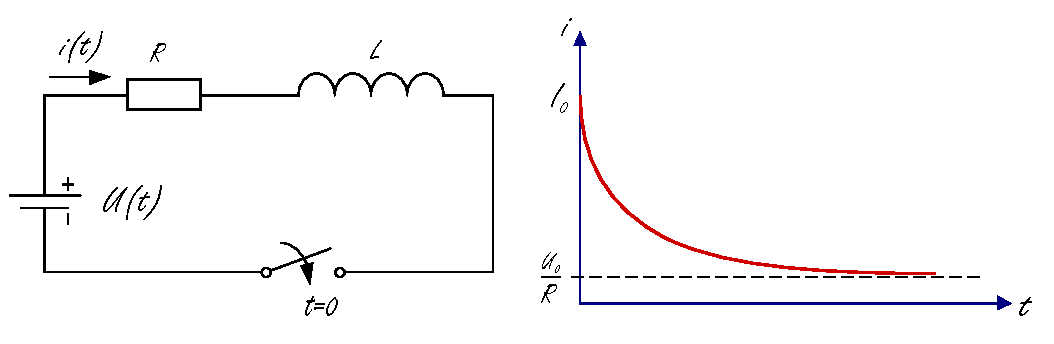
\includegraphics[width=\linewidth]{mai_fig032.pdf}
      \caption{Graf průběhu proudu $i(t)$ po sepnutí spínače v době $t=0$.}
      \label{mai:fig032}
    \end{figure}
%---------------------------------------------------------------------------------------------------